\documentclass[a4paper,twocolumn]{article}

\usepackage[english]{babel}
\usepackage[utf8]{inputenc}
\usepackage{graphicx}
\usepackage{hyperref}
\usepackage{fullpage}
\usepackage[small]{titlesec}

% patch titlesec bug of not showing (sub)title numbering http://tex.stackexchange.com/a/300259
\usepackage{etoolbox}
\makeatletter
\patchcmd{\ttlh@hang}{\parindent\z@}{\parindent\z@\leavevmode}{}{}
\patchcmd{\ttlh@hang}{\noindent}{}{}{}
\makeatother


\newcommand*\mean[1]{\overline{#1}}

\title{The Cascade-Correlation Learning Architecture $-$ summary}
\author{Matěj Nikl}

\begin{document}
\maketitle
\noindent
The Cascade-Correlation Architecture (CCA) is a architecture as well as a supervised learning algorithm for artificial neural networks (ANNs). Conventional way of training ANNs is to \textit{somehow} choose a fixed network topology and then train it using back-propagation algorithm.
CCA eliminates the need of choosing a fixed network topology and provides a way of training this kind of a dynamic network.

\section{Principles of growing}
The network starts with no hidden units, only output units are present. Then, one hidden unit is added at a time, receiving all network inputs and all outputs of the previously added hidden units, each time adding more complexity to the network, possibly creating more and more complex feature detectors.

\begin{figure}[!h]
    % \centering
    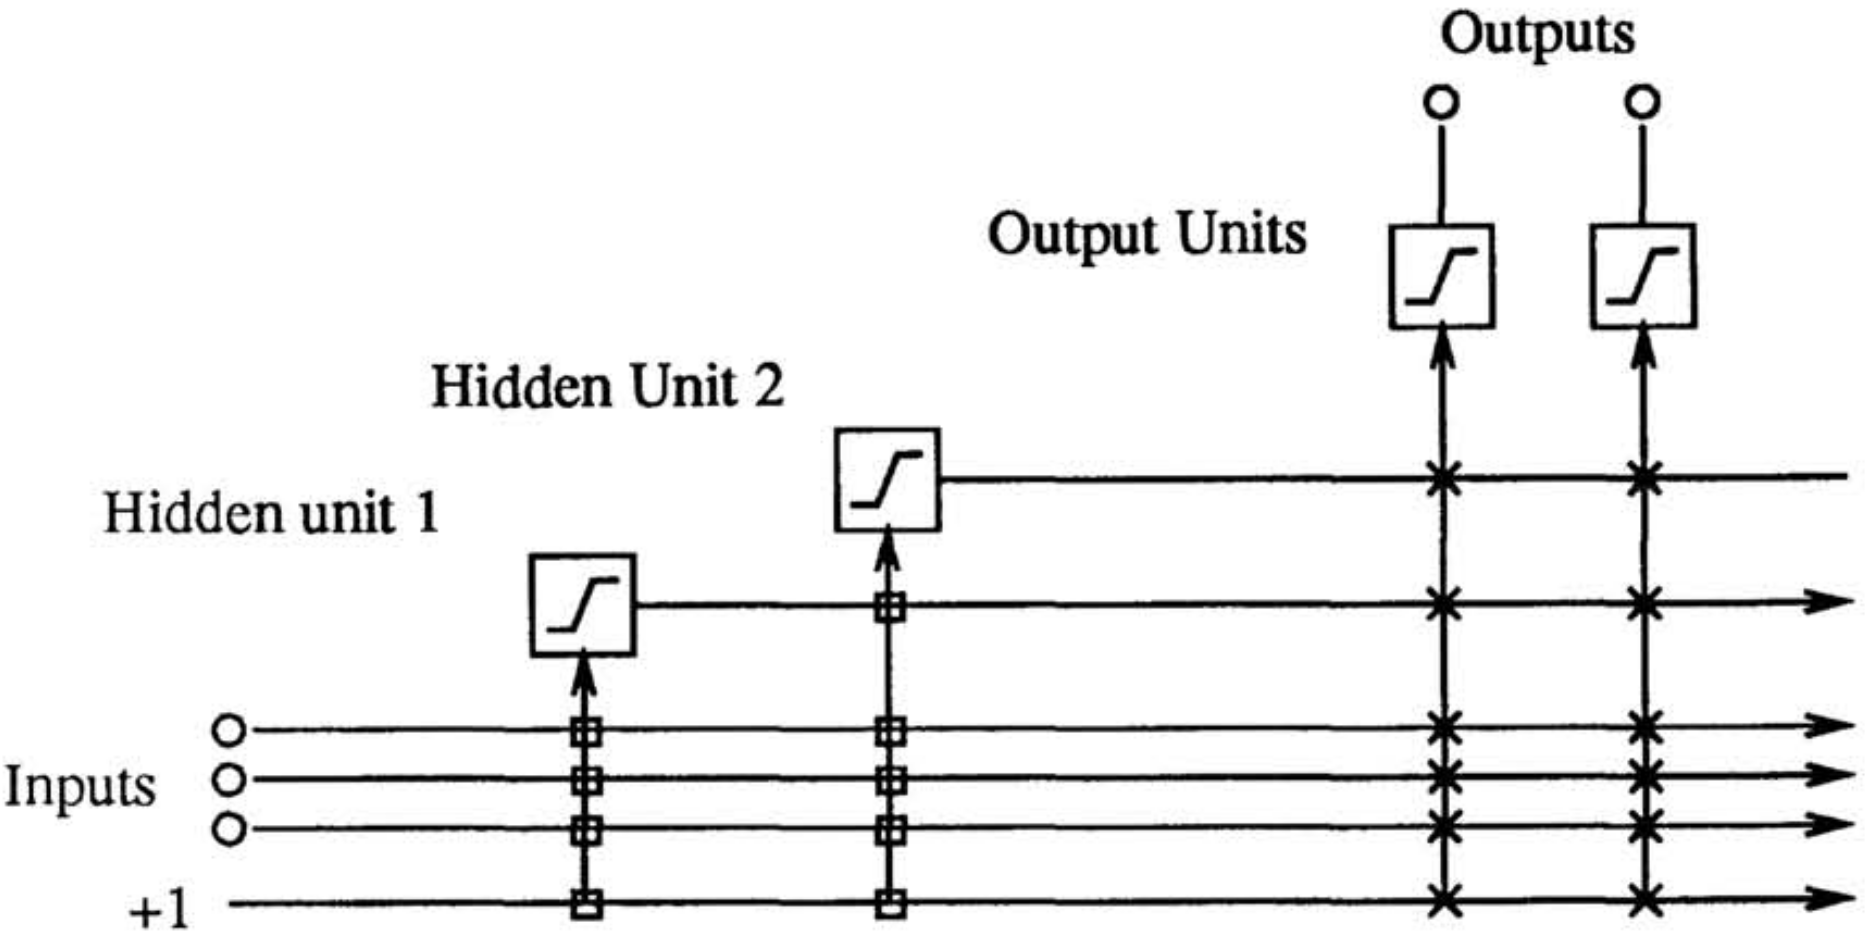
\includegraphics[width=0.475\textwidth]{cascade.png}
    \caption{The CCA after two hidden units have been added. The vertical lines sum all incoming activations. Boxed connections are frozen, X connections are trained repeatedly.}
\end{figure}

\section{Training}
The process of training can be divided into two parts, which will be described in the following subsections, however one constraint holds through both of them: once a new hidden unit is added, its input weights are forever frozen.
% \begin{itemize}
%     \item \ref{ssec:nn} training the network output
%     \item \ref{ssec:unit} training a new hidden unit, to-be added to the network
% \end{itemize}
\subsection{Network output training} \label{ssec:nn}
Having everything except output units' weights frozen translates into optimization of a single layer network, which was one of the authors' goals (to avoid slow back-propagation). The following steps take place:
\begin{enumerate}
    \item optimize the single layer network, until a convergence is achieved
    \item evaluate the test error and if it is low enough, stop
    \item otherwise, proceed to subsection \ref{ssec:unit}
\end{enumerate}

\subsection{New unit training} \label{ssec:unit}
If network's test error is not low enough, we need to add a new hidden unit. To do so, the following steps take place:
\begin{enumerate}
    \item create a pool of \textit{candidate} units, having their input weights randomly initialized, each receiving all available inputs
    \item maximize $S$, the sum of covariances between the candidate unit's value and the residual output error of all output units, for each candidate unit, by adjusting their input weights, until convergence
\[
    S = \sum_{o \in O} \left| \sum_{p \in P} (V_p - \mean{V})(E_{p,o} - \mean{E_o}) \right|
\]
    \begin{itemize}
        \item $O$ is a set of output units
        \item $P$ is a set of training patterns (training data)
        \item $V_p$ is candidate unit's value for pattern $p$
        \item $E_{p,o}$ is the residual output error at output unit $o$ for pattern $p$
        \item averages are computed across $P$
    \end{itemize}

    \item choose the candidate unit with the largest $S$ and add it to the network, proceed to \ref{ssec:nn}
\end{enumerate}

\section{Principles of modularization}
The only sense of modularization in the CCA can be seen in viewing individual hidden units as modules, since they are being added throughout the learning process. However, the network as a whole is not modular in the full sense. Hidden units cannot be detached from a network and reattached to a different one. A hidden unit can only be used in conjunction with the hidden units it has been trained with and nowhere else.
\paragraph{Similar design}
A similar partially modular design can be seen in Progressive Neural Networks, where new columns (full-blown NNs) are being added with lateral connections to all of the previously trained columns, showing the same aspects of \textit{(non)modularity} as CCAs.


\end{document}
